\chapter{Design}
\section{Architectural design}
In this section we will define the architecture of the entire system, showing the dependencies between its components. See Figure 4.1.

\begin{figure}
\noindent\makebox[\textwidth]{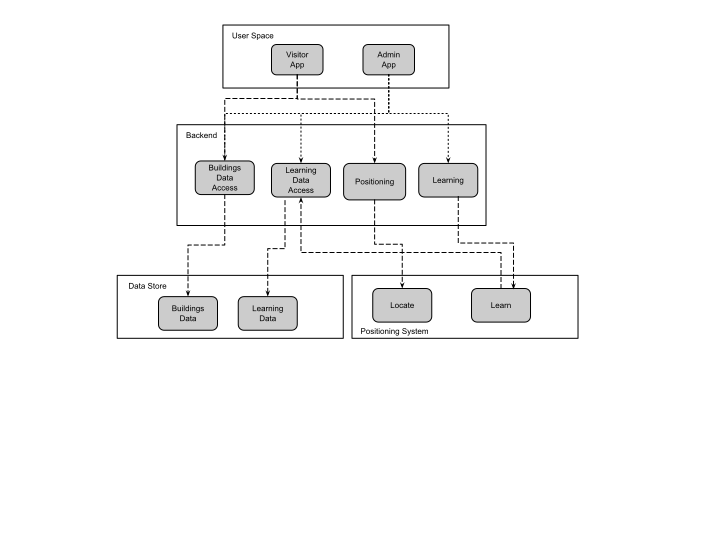
\includegraphics[clip, trim=0cm 3cm 0cm 0.7cm, width=\paperwidth]{DIAGRAMS/SystemArch.pdf}}
\caption{System Architecture}
\end{figure}
The architecture of the system is comprised of three subsystems. The top subsystem is concerned with interfacing the end users (HOST and VISITOR) to the lower subsystems. The middle subsystem offers an API to the bottom subsystems. The bottom subsystems manage and provide the information required for the entire system to run. To continue, we will review each subsystem in more detail, from top to bottom.
\clearpage
\subsection{User Space}
This layer is comprised of two Android Application, one for each type of user.
\\
The following are common features for both applications:
\begin{enumerate}
\item Implement serializable classes for the models defined in the database
\item Request and receive data from the backend in JSON format.
\item Post data to the Backend in JSON format.
\item Parse JSON data to create Java Objects
\item Convert Java Objects into JSON.
\item Activity to display all the buildings available in a ListView
\item Buildings ListView must be clickable and, on click should launch another activity for the specific building.
\item Clicking on a room should launch an activity for the selected room.
\item Implement Wi-Fi capabilities in order to measure signal strength of all visible APs.
\end{enumerate}
These common features will be implemented in packages that can be shared across the two apps.
\\
\textbf{Administration application (HOST)}
\\
Due to the difference in requirements a separate android application must be developed for the HOST. In addition to the common features, the application will also implement the following:
\begin{enumerate}
\item A button to add a new building In addition to the list of available buildings.
\item An add building activity containing a form and a submit button for creating a new building
\item Selecting a building from the list opens an activity containing fields that can be used to edit the building’s information.
\item A clickable ListView with all rooms in a building as part of the activity mentioned above.
\item A "learn" button to update the Positioning system with new data.
\item Clicking on an item in the Rooms ListView will open an activity that will allow the apps to measure the signal strength of all APs, associating them with the selected room, posting to the database.
\item A button in the Building activity to add new rooms.
\item The add room button will open an activity containing a form and a submit button for creating a new room.
\end{enumerate}

\textbf{Visitor application}
\\
In addition to the common features, the visitor application will also implement the following:
\begin{enumerate}
\item A clickable ListView with all the buildings available.
\item Selecting a Building will open an activity containing a list of all rooms as selectable items. Selecting an item will update the Estimated Time value displayed somewhere below.
\item A button to start the visit will open another activity that either displays the Google Indoor Map if available, or a textview.
\item The Visit Activity displays the current location of the visitor as a pin on the Map or as text.
\item The Visit Activity will also display a recommended path for the visit on the Map or as text.
\end{enumerate}

\subsection{Backend}
For the simplicity of the software, and for a more efficient integration of all subsystems, the backend is ran using a NodeJS server, implementing a RESTful API.
The API handles HTTP methods to "http://serveraddress/res/", where res is the resource targeted. In addition /res/id can be used, where available, to apply method to a resource that has the specified id.
The resources available and the results of each method are as follows:
\begin{itemize}
\item For resource "buildings/":
	\begin{itemize}
	\item GET: Returns a list of all buildings stored in the database
	\item POST: Adds a new building to the database
	\end{itemize}
\item For resource "buildings/id/":
	\begin{itemize}
	\item GET: Returns the building with the specified id
	\item PUT: Updates the building with the specified id
	\item DELETE: Deletes the building with the specified id
	\end{itemize}
\item For resource "rooms/id/":
	\begin{itemize}
	\item GET: Returns the rooms that belong to the building with the specified id
	\item POST: Adds a new room to the building with the specified id
	\item DELETE: Deletes the room with the specified id
	\end{itemize}
\item For resource "measurements/":
	\begin{itemize}
	\item GET: Returns all measurements taken on the system
	\item DELETE: Deletes all measurements taken on the system
	\end{itemize}
\item For resource "measurements/id":
	\begin{itemize}
	\item GET: Returns measurements taken for the room with the specified id
	\item POST: Adds a new measurement associated to the room with the specified id
	\end{itemize}
\item For resource "learn/id":
	\begin{itemize}
	\item GET: Updates the positioning system for the building with the specified id
	\end{itemize}
\item For resource "locate/id":
	\begin{itemize}
	\item POST: Returns the predicted location in the building with the specified id
	\end{itemize}
\item For resource "route/id":
	\begin{itemize}
	\item POST: Returns the generated route, based on the requirements sent, through the building with the specified id
	\end{itemize}
\end{itemize}

\subsection{Positioning System}
This is the most important part of the project. It is the software which implements the machine learning and data processing algorithms in order to create the classifiers needed for positioning.
This subsystem is built out of a X modules, each one with its own task. It is implemented using the Weka Machine Learning libraries. The software implements the following features:
\begin{enumerate}
\item Opens TCP connections in order to receive requests and data.
\item A JSON Object is received containing the request type and the data to be used.
\item For a request of type "learn" the software parses the data received and creates a classifier using it.
\item In order for this to happen, the software will require to convert the data into and ARFF file format.
\item A list of all the rooms is extracted and saved as a local file in JSON format. The file is named using the "building\_id"+"\_buildings.json"
\item A list of all the Reference Points (RPs) is extracted and saved as a local file in JSON format. The file is named using the building\_id + \_RPs.json
\item Using the learning set ARFF file, a classifier is initialised and added to an array for future use.
\item For a request of Type "classify", the system checks whether a classifier has been built for the building id given in the request.
\item If a classifier has been previously built but it has not been initialised in the current run of the system, the server will initialise a classifier using the data saved from the previous learn command called for the building.
\item If a classifier has never been built, the system will return an error.
\item Once the classifier is initialised, it will be used to classify the data received in the request, and will return the room as a result.
\item The system implements multiple algorithms therefore a format must be implemented to return multiple results given by different algorithms. The data is returned as follows: [algorithm\_name]:[predicted\_room\_id],[algorithm\_name]:[predicted\_room\_id], etc. In other words, the algorithm name and the room predicted by it are separated by ":" and the algorithms are separated using ",".
\item For a request of Type "route", the system parses the requirements in JSON and creates a problem file in PDDL. 
\item The problem file is then used with the predefined domain file and the OPTIC planner to generate a suggested route.
\item The data returned by the planner must also be parsed, the resulting data to be sent following the pattern:
 "view:room1;walk:room1,room2;view:room2" etc.
\end{enumerate}

\textbf{Prediction System:}
\\
When designing the system, multiple methods for finding the location of the device were considered.
\\
\textit{\textbf{Trilateration}}
\\
Firstly, dimensions of the building and its rooms, and the coordinates of each RP must be known. An RSS measurement is then taken for each visible RP: one next to the RP and one at the furthest corner from the RP, in the same room. To increase precision, more measurements at each of the two points can be taken and the results averaged. \\ 
We define: \\
$MRP_0$ - Average signal strength taken at the RP coordinates. \\
$MRP$ - Average signal strength taken at the furthest corner from the RP, in the same room. \\
$DRP$ - Distance (in meters) from the RP's location to where $MRP$ was taken.\\
In perfect conditions the Distance as a function of Signal Strength increases linearly. Therefore, to convert Signal Strength to Distance is a regression problem.\\
Using the equation of the line $$y = mx + n$$ we must find the gradient $m$ and the y-intercept $n$.\\
We compute $$m = \frac{DRP}{MRP - MRP_0}$$
and $$n  = DRP - m * MRP$$
$m$ and $n$ values are then saved for each RP and the distance will be calculated as $$Distance  = M * RSS + N$$
\\
To find the location of the device based on the distance measured we must find the intersection of $n$ circles (where $n$ is the number of RPs taken into account and must be greater than 3 if the coordinates must be found in 2 dimensional space, or 4 if in a 3 dimensional space).  To determine the intersection points for 3 RPs we will use the algorithm defined by Paul Bourke [8]:\\
First calculate the distance d between the center of the circles $d = |P_1 - P_0|$\\
If $d > r_0 + r_1$ or $d < |r_0 - r_1|$ then there are no solutions. If $d = 0$ and $r_0 = r_1$ then are an infinite number of solutions.\\
Considering the two triangles $P_0P_2P_3$ and $P_1P_2P_3$ we can write $$a^2 + h^2 = r_0^2$$ $$b^2 + h^2 = r_1^2$$

Using $d = a + b$ we can solve for $a$,
$$a = \frac{r_0^2 - r_1^2 +d^2}{2d}$$
It can be readily shown that this reduces to $r_0$ when the two circles touch at one point.
Solve for $h$ by substituting a into the first equation, $$h^2 = r_0^2 - a^2$$
So $$P_2 = P_0 + \frac{P_1 - P_0}{d}$$
And finally, $P_3 = (x_3, y_3)$ in terms of $P_0 = (x_0, y_0),  P_1 = (x_1, y_1) and P_2 = (x_2, y_2)$ is $$x_3 =\frac{x_2 + -h(y_1 - y_0)}{d}$$ $$y_3 =\frac{y_2 - +h(x_1 - x_0)}{d}$$
The problem with this approach is that it assumes that the distance measurements are precise. In our case, where the readings are not precise, errors can occur, such as one or more circle not intersecting in one exact point or, intersecting at all.
This can be solved by finding the closest point to all circles, such that the sum of all distances from a point to the circle be the minimum.\\
\\
\textit{\textbf{Probability based approach}}
\\
Because the specification of the software favours precision over accuracy, it is therefore a better approach to try and guess the room in which the device is found, instead of the actual coordinates. Therefore, an approach is to calculate the probability of a device to be in a room, based on statistic data.\\
Each room must store a list of average readings for all the reference points visible from that room. 
We define:\\
\begin{itemize}
\item $AVG(RP_x, R_y)$ as the average signal strength value for $RP_x$ taken in room $R_y$.
\item $N(R_y)$ as the number of RPs that can be measured from room $R_y$.
\item $mRP_x$ as a signal strength measurement for $RP_x$.
\end{itemize} 

A reading is given as a list of $mRP$, that is, the readings taken at a moment in time. The goal is to use this list and calculate the probability that the readings were taken in a specific room.\\
For each room $R_i$, we calculate $S$ for each measurement $mRP_j$, if $AVG(RP_j, R_i)$ exists and is different than 0, as follows:
$$S(RP_j, R_i) = | 1 - \frac{mRP_j}{AVG(RPj, Ri)}|+1$$
Giving us a score from 1 to infinity.\\
We then calculate 
$$\frac{\displaystyle\sum_{i=1}^{M} \frac{1}{S(RP_i, R_x)}}{N(R_x)}$$
where $M$ is the number of measurements in the set.
The result is the probability for the measurements to have been taken in room $R_x$.
We can then compare the probability for all rooms and choose the one which is most likely.
\\
\textit{\textbf{Machine Learning approach}}
\\
Machine Learning algorithms can be applied to this application in order to predict the room in which a device is located. We first define a learning set of all measurements taken and the rooms that the measurements were taken in.\\
There are five classifiers considered:
Naive Bayes, Bayes Networks, KStar, Decorate and NB Trees. The classifiers are implemented using the Weka Machine Learning Library. The result of each classifier is returned to the backend, therefore, the decision of which predicted value to be used is moved higher up in the system.
Due to a higher level of precision, the Machine Learning approach will have the priority in implementation.

\subsection{Data Store}
The Data Store contains two types of data, Building related and Learning related. 
Building data is all data concerning the operation and visualisation of the buildings and the rooms contained. Learning data is the data used by the Positioning System.
Initially, this layer was designed using an MySQL, but due to compatibility and performance issues with Android and longer development time, it has been changed to MongoDB.
\\
The following data models were defined to be used with the database:
\\
RECTANGLE:	
\begin{itemize}
	\item 4 coordinates (X,Y), one for each angle: Left-top (LT), Right-top (RT), Left-bottom(LB), Right-bottom (RB)
\end{itemize}

BUILDING:
\begin{itemize}
	\item Name: The name of the building as a string.
	\item Rectangle: The rectangle model that defines the building.
	\item Width and Height(length)
\end{itemize}


ROOM: 
\begin{itemize}
	\item Name: The name of the room as a string.
	\item Rectangle: The rectangle model that defines the room.
	\item Width and Height(length)
	\item Floor: The floor number in which this room is located.
	\item Estimated Time of Visit
	\item Building ID: to associate each room to a building
\end{itemize}

Reference Point (RP): This is a point in space for which distance measurements are taken.
\begin{itemize}
	\item RPID: A unique identifier
	\item Building ID: To associate each RP to a building.
	\item Coordinates (X, Y)
\end{itemize}

RP Measurement: Distance to an RP as measured in a specific room.
\begin{itemize}
	\item RP - Value Pair: Contains the RPID and the value of the measurement
	\item Room ID: The ID of the room in which the measurement was taken
\end{itemize}

\section{DATA FLOW and STATE MACHINE}
Because of the vast amount of data that must be transferred between the subsystems, it is important to visualise and understand what data must be inputted in each subsystem, what data is outputted by each subsystem and how this data moves around in the entire system.
\begin{figure}
\noindent\makebox[\textwidth]{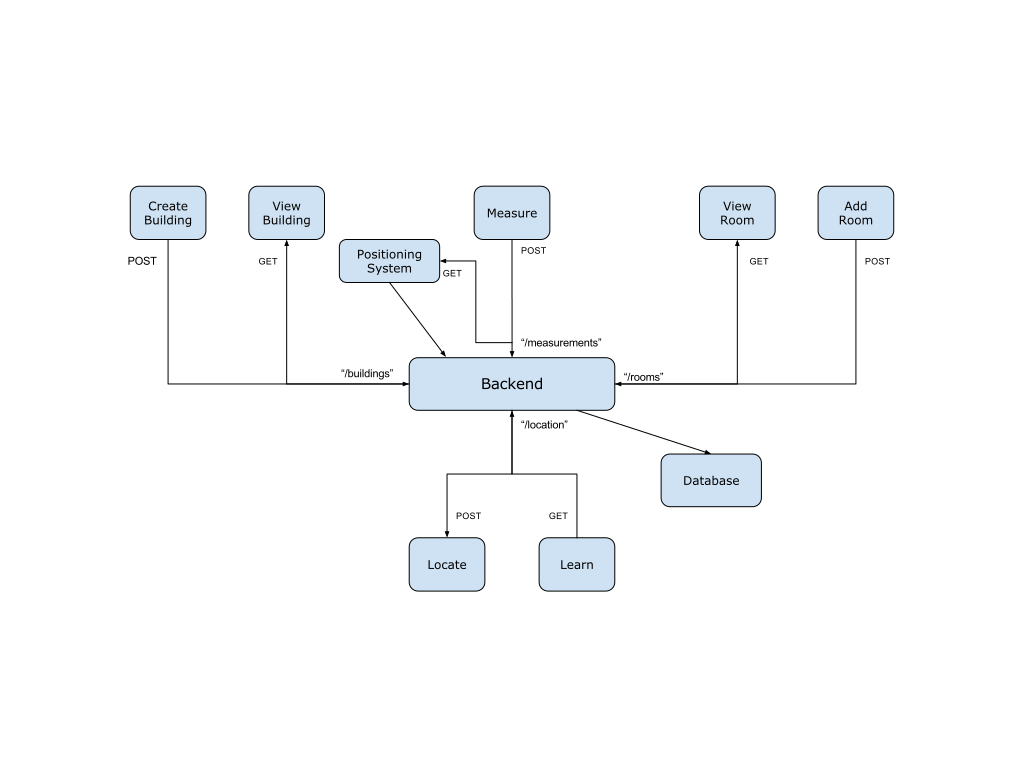
\includegraphics[width=\paperwidth]{DIAGRAMS/dataflow.pdf}}
\caption{Data Flow}
\end{figure}
The initial input is in the HOST android application. Here, the user inputs the details of a new building to be created. The data is then converted into JSON and sent to the Backend through a POST request to "/buildings". The backend parses the data and creates a new Building object, storing it in the database. The HOST then can select the building created and begin adding new room. For each new room, the details are entered and submitted. After submitting each room, the data, in JSON format, is sent to the Backend using a POST request to "/rooms/building\_id". The backend then created a new Room object, setting its building id to the specified id and storing it in the database. After the required rooms are added, the HOST must then take the RSS measurements for each room, in order for the classifier to be built. In the room activity, the HOST starts the measurements, and a list of all measurements taken at a point in time is then sent to the backend through a POST method to "measurements/room\_id", where the backend stores it in the database.
After enough measurements were taken for all the rooms, the host can then press the "learn" button from the building activity, which will send a GET request to "/locate/building\_id". On receipt of this request, the backend queries the database for all the measurements taken in the building and sends it through a TCP connection to the Positioning system, as a "learn" request. The positioning system processes the request and data, parsing it and storing the data locally. It will then initialise a classifier using the data stored, the system is then in standby again. \\
The next trigger is made by the VISITOR app, which, on start, will request a list of buildings from the backend using GET "/buildings/". The backend the queries and returns all the buildings stored. The user can then press on a building and see the list of rooms available. When the user starts a visit, a POST request is sent with the rooms and "want" levels that the user has specified to "/route/". The backend then sends a "route" request and forwards the data to the positioning system, which returns the suggested route. Finally, the app starts collecting RSS measurements. For every scan, the list of measurements is sent to the backend using a POST request to "/locate/building\_id". This triggers the backend to send a "classify" request to the positioning server, which returns a list of predicted locations. The backend the forwards the information back to the user.

